\documentclass{article}
\usepackage{graphicx}
\usepackage{wrapfig}

\begin{document}

\begin{wrapfigure}{l}{0.17\textwidth}
  \includegraphics[width=0.18\textwidth]{Melkamu Mersha.jpg}
\end{wrapfigure}

\noindent % Prevents paragraph indentation
Melkamu Mersha earned his BSc and MSc degrees in Computer Science from the University of Gondar, Ethiopia. He is currently pursuing a Ph.D. in Computer Science at the College of Engineering and Applied Science, University of Colorado, Colorado Springs. His research primarily focuses on Artificial Intelligence, specifically, eXplainable Artificial Intelligence (XAI), Machine Learning, and Natural Language Processing (NLP).

% \vspace{2mm}

\begin{wrapfigure}{l}{0.17\textwidth}
  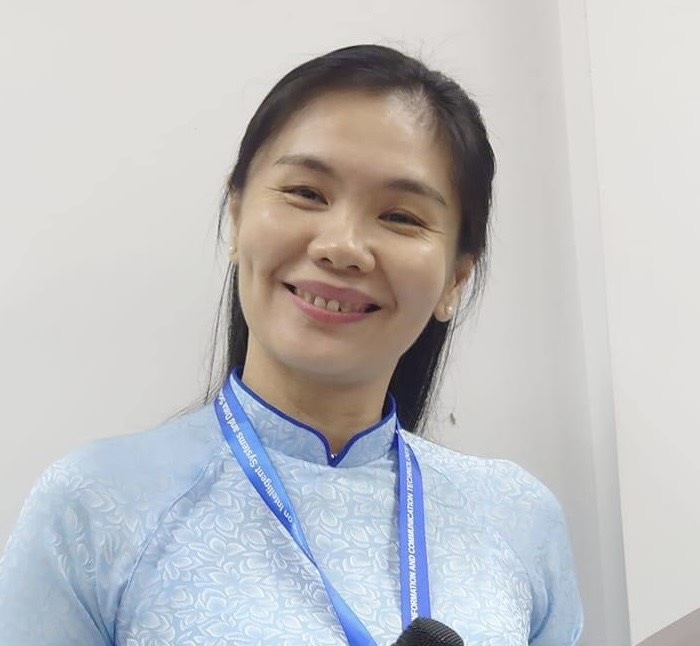
\includegraphics[width=0.18\textwidth]{KhangLam.jpg}
\end{wrapfigure}

\noindent
Dr. Khang Lam received the Bachelor’s degree in Computer Science from Can Tho University, Vietnam, in 2005, the Master’s degree in Information Technology from Ewha Womans University, South Korea, in 2009, and the Ph.D. degree in computer science from the University of Colorado, Colorado Springs, USA, in 2015. Since 2015, she has been a Senior Lecturer with the Department of Information Technology, Can Tho University. Her research interests include Natural Language Processing, Question-Answering systems, Image Captioning, and Deep Learning.

% \vspace{2mm}

\begin{wrapfigure}{l}{0.17\textwidth}
  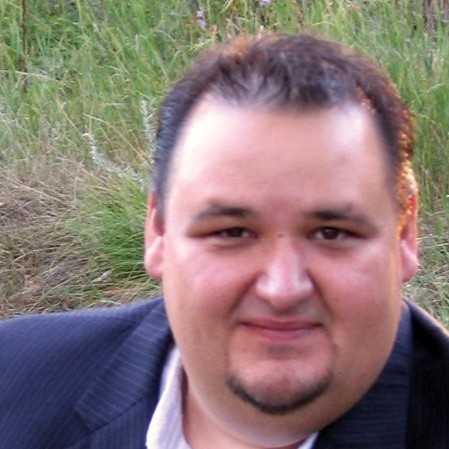
\includegraphics[width=0.18\textwidth]{Joseph.jpeg}
\end{wrapfigure}

\noindent
Joseph Woods holds a Bachelor of Science in Chemical Engineering, a Master's degree in Applied Physics focusing on theoretical magnetism, and is currently pursuing a Ph.D. in Artificial Intelligence. Their research centers on applying deep learning techniques to identify skyrmions in magnetic solutes under external magnetic fields, aligning with their long-term goal of merging fundamental science with machine learning. Additionally, they are actively involved in researching Explainable Artificial Intelligence (XAI), aiming to enhance transparency and interpretability in complex AI models, addressing both scientific and societal concerns surrounding AI ethics and accountability.

% \vspace{20mm}

\begin{wrapfigure}{l}{0.17\textwidth}
  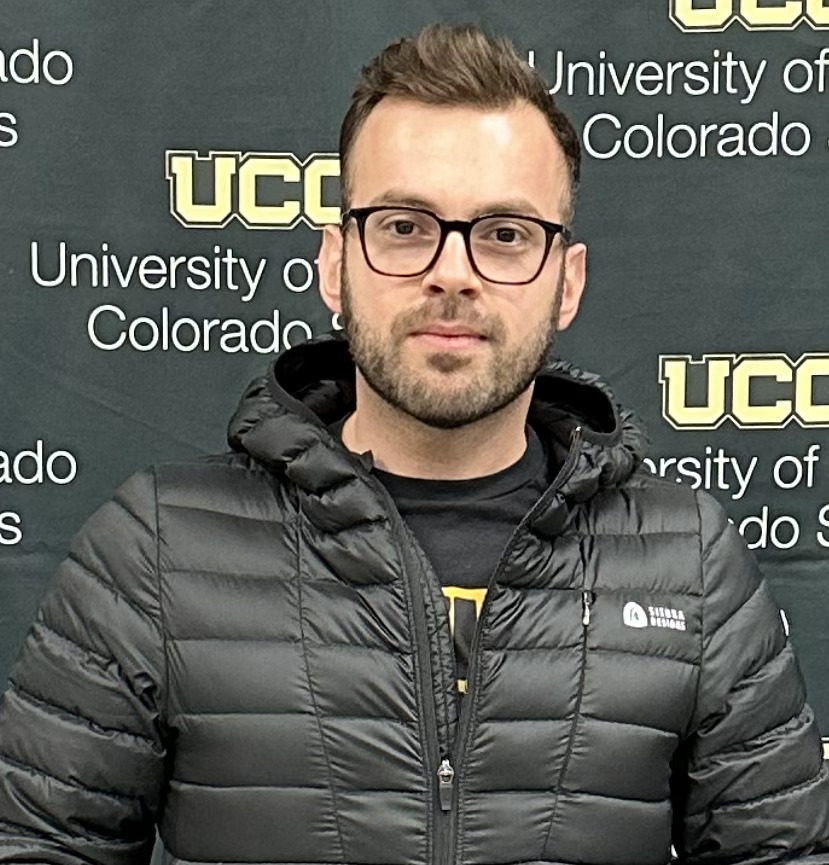
\includegraphics[width=0.18\textwidth]{AlShami.jpg}
\end{wrapfigure}

\noindent
Ali AlShami is a Ph.D. candidate in the Computer Science Department at the University of Colorado, Colorado Springs (UCCS). He earned his Master's degree from the same institution in 2021. Computer Vision and Machine Learning are areas of research interest. Specific areas include image classification, segmentation, human pose estimation, human action recognition, human trajectory prediction, object detection, SVO interaction, and open-set recognition.

\vspace{2mm}

\begin{wrapfigure}{l}{0.17\textwidth}
  \includegraphics[width=0.18\textwidth]{Kalita.jpg}
\end{wrapfigure}

\noindent
Dr. Jugal Kalita earned his Bachelor of Technology degree from the Indian Institute of Technology in Kharagpur, India. He received his Master of Science degree from the University of Saskatchewan, Canada, and a Master of Science and a Ph.D. from the University of Pennsylvania. He teaches a variety of classes, having taught almost 20 different classes during his career at UCCS. His research interests include artificial intelligence and machine learning, with a particular focus on deep learning, bioinformatics, and computer security.

\end{document}
